%!TEX root = ../thesis.tex

\cleardoublepage
\chapter{Technologies and Concepts of a Larger Context}

This appendix chapter contains definitions for technologies and concepts that are mentioned in the thesis, but are not of higher importance for it. Section \ref{sec:paxos} introduces a consensus algorithm for distributed systems.

\section{Finding Consensus in a Distributed System}
\label{sec:paxos}

The Paxos algorithm has first been described by Leslie Lamport in their work about the parliament on the island of Paxos \cite{paxos1998}.
The parliament's part-time legislators had been able to maintain consistent copies of their records by following the algorithm protocol.
While the original work's main focus has not been the application in computer science, the author simplified their explanations later in \cite{paxos2001} and described how Paxos can be used to find consensus in fault-tolerant distributed systems.

Even though the Paxos algorithm cannot mitigate Byzantine failures (see appendix \ref{app:dic}), it can mitigate the effects of different processing speeds of participants and reordered, delayed, or lost messages.
The only requirement is that at least half of the participants can somehow communicate.

In Paxos, four different roles exist. The \textbf{client} issues requests and waits for responses.
Based on the client's request, multiple \textbf{proposer} propose a value. All these proposals are processed by the \textbf{acceptors} which will agree upon one at the end.
Finally, there are the \textbf{learners} which guarantee persistence of agreed decisions and respond to client reads.
The usual setup used in practice, in which every machine participating fulfills each of the roles besides the client role, is shown in figure \ref{fig:paxosSetup}.

\begin{figure}[ht]
    \centering
	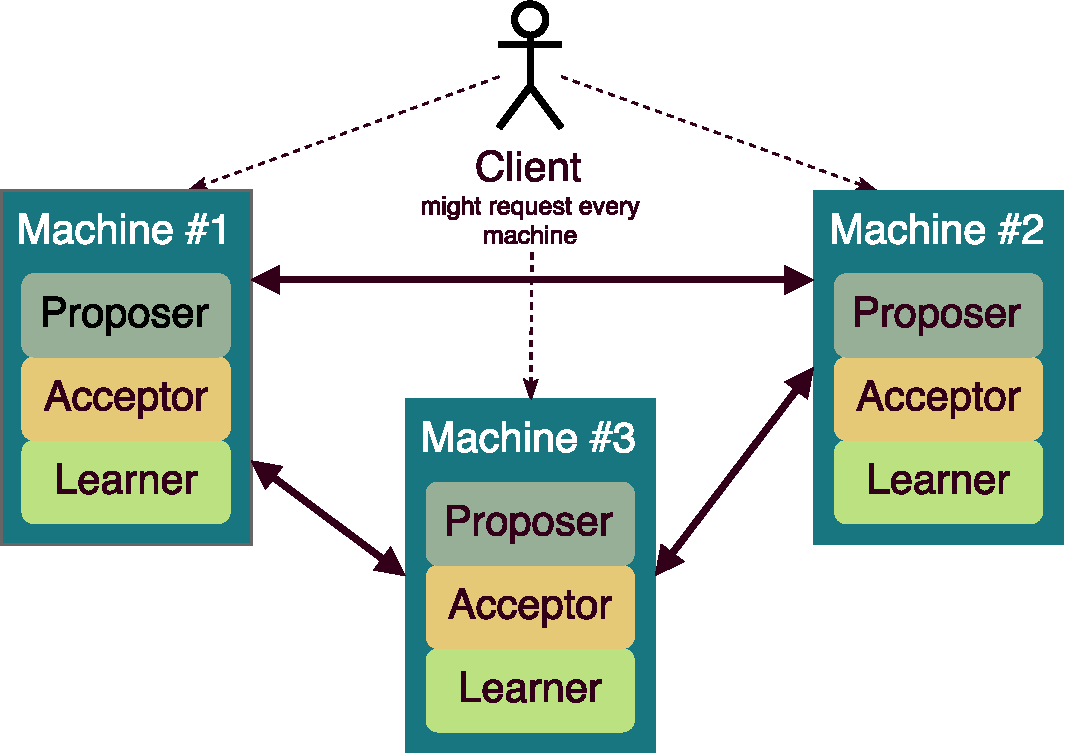
\includegraphics[width=0.8\textwidth]{fig/PaxosSetup.pdf}
	\caption{Example Setup of Three Machines Agreeing on Values Based on the Paxos Algorithm}
	\label{fig:paxosSetup}
\end{figure}

\section{Detecting Mutual Inconsistency}
\label{sec:versionVector}

Parker et al. claim that a system must ensure the mutual consistency of data copies by applying all changes made to one copy to all others correspondingly \cite{versionVektor}.
Each time two copies of the same original data item have a different set of modification applied to them, they become incompatible and this conflict must be detected.
However, this is not trivial, because \enquote{network partitioning can completely destroy mutual consistency in the worst case}.
Nevertheless, Parker et al. state that the efficient detection of conflicts that lead to mutual inconsistency can be done by a concept they call \textit{version vectors}.
They define a version vector for an item f as \enquote{a sequence of n pairs, where \textit{n} is the number of sites at which f is stored. The \textit{i}th pair ($S_i$: $v_i$) gives the index of the latest version of \textit{f} made at site $S_i$}.
An example vector for an item stored at the sites A, B and D is $<$A:2, B:4, D:3$>$, which translates in a file that has been modified twice on site A, four times on site B, and thrice on site D.

A set of vectors is \enquote{compatible when one vector is at least as large as any other vector in every site component for which they have entries}.
Otherwise the vectors conflict and are incompatible.
E.g., the two vectors $<$A:2, B:4, D:3$>$ and $<$A:4, B:5, D:3$>$ are compatible because the second one dominates the other one.
$<$A:3, B:4, D:3$>$ and $<$A:2, B:5, D:3$>$ conflict, because the first one indicates that the data item was modified one more time on node A, while the second one indicates one more modification occurred on node B.
However, if we add a third vector $<$A:3, B:5, D:4$>$, no conflict exists anymore, because it dominates the two others.
The consequences of an operation performed on a data item for a data item's vector is depicted in table \ref{tab:vectorOperations}.

\begin{table}[ht]
    \centering
    \begin{tabularx}{\linewidth}{@{}>{\bfseries}l@{\hspace{.5em}}X@{}}
        \toprule
        \textbf{Operation related to data item} & \textbf{Consequence for vector of data item}\\ \midrule
        Update on site $S_i$ & Increment $v_i$ by one\\
        Delete or rename on site $S_i$ & Keep vector and increment $v_i$ by one, remove data item value\\
        Reconcile version conflict & Set each $v_i$ to maximum $v_i$ from all vectors used for reconciliation. In addition, increment $v_i$ of site that initiated reconciliation by one\\
        Copy to new site & Augment vector to include new site\\
        \bottomrule
    \end{tabularx}
    \caption{Influence of Operations on a Data Item's Version Vector}
    \label{tab:vectorOperations}
\end{table}

By using version vectors, one can detect version conflicts and initiate (automatic) reconciliation.
However, Parker et al. warn that two identical updates made on separate partitions will result in a conflict, even though none is present.
Thus, they recommend to additionally check two data items on differences before a conflict is raised in certain applications.
Furthermore, the reconciliation is most times not trivial, that's why tools such as Cassandra delegate this task to the application layer \cite{cassandra2010}.
